\documentclass[dvipsnames]{beamer}

\usepackage[utf8]{inputenc}
\usepackage{url}
\usepackage{amssymb}
\usepackage{amsmath}
\usepackage{amsbsy}
\usepackage{mathbbol}
\usepackage{mathtools}

% Diagrams
\usepackage{tikz}

% Mathbb doesn't support digits
\usepackage{bbm}

% Example code
\usepackage{listings}

% Inference rules
\usepackage{mathpartir}

% Multiple columns
\usepackage{multicol}

% Newline inside table
\usepackage{makecell}

% Square bullet points
\newcommand{\sitem}{\item[\raisebox{.45ex}{\rule{.6ex}{.6ex}}]}

% Abbreviations
\newcommand{\lambdacalc}{$\lambda$-calculus}
\newcommand{\picalc}{$\pi$-calculus}
\newcommand{\Picalc}{$\pi$-Calculus}

% Typing rules
\newcommand{\stacked}[1]{\mprset{flushleft} \inferrule*{}{#1}}
\newcommand{\datatype}[2]{{\mprset{fraction={===}} \inferrule{#1}{#2}}}

\newcommand{\type}[1]{\textcolor{BlueViolet}{\operatorname{#1}}}
\newcommand{\constr}[1]{\textcolor{BurntOrange}{\operatorname{#1}}}
\newcommand{\func}[1]{\textcolor{OliveGreen}{\operatorname{#1}}}

% Constructors
\newcommand{\PO}{\constr{\mathbb{0}}}
\newcommand{\comp}[2]{#1 \; \constr{\parallel} \; #2}
\newcommand{\new}{\constr{\boldsymbol{\nu}} \;}
\newcommand{\send}[2]{#1 \; \constr{\langle} \; #2 \;\constr{\rangle} \;}
\newcommand{\sendp}[2]{#1 \; \constr{\langle} \; #2 \; \constr{\rangle} \; . \;}
\newcommand{\recv}[1]{#1 \; \constr{\mathbb{()}} \;}
\newcommand{\recvp}[2]{#1 \; \constr{(} \; #2 \; \constr{)} \; . \; }
\newcommand{\suc}{\constr{\scriptstyle 1+}}
\newcommand{\unit}{\constr{\mathbbm{1}}}
\newcommand{\base}[1]{\constr{B[} \; #1 \; \constr{]}}
\newcommand{\channel}[2]{\constr{C[} \; #1 \; \constr{;} \; #2 \; \constr{]}}
\newcommand{\comma}{\; \constr{,} \;}

% Functions
\newcommand{\subst}[3]{#1 \; \func{[} \; #3 \; \func{\mapsto} \;#2 \; \func{]}}
\newcommand{\op}[3]{#1 \; \func{\coloneqq} \; #2 \; \func{\cdot} \; #3}
\newcommand{\opsquared}[3]{#1 \, \func{\coloneqq} \, #2 \, \func{\cdot^2} \, #3}
\newcommand{\opctx}[3]{#1 \, \func{\coloneqq} \, #2 \, \func{\otimes} \, #3}
\newcommand{\zero}{\func{0\cdot}}
\newcommand{\one}{\func{1\cdot}}
\newcommand{\li}{\func{\ell_i}}
\newcommand{\lo}{\func{\ell_o}}
\newcommand{\lz}{\func{\ell_{\o}}}
\newcommand{\lio}{\func{\ell_{\#}}}

% Types
\newcommand{\Set}{\type{SET}}
\newcommand{\reduce}[1]{\; \type{\longrightarrow}_{#1} \;}
\newcommand{\types}[4]{#1 \; \type{;} \; #2 \; \type{\vdash} \; #3 \; \type{\triangleright} \; #4}
\newcommand{\contains}[6]{#1 \; \type{;} \; #2 \; \type{\ni}_{#3} \; #4 \; \type{;} \; #5 \; \type{\triangleright} \; #6}
\newcommand{\containsusage}[4]{#1 \; \type{\ni}_{#2} \; #3 \; \type{\triangleright} \; #4}
\newcommand{\Var}{\type{VAR}}
\newcommand{\Process}{\type{PROCESS}}
\newcommand{\Unused}{\type{UNUSED}}
\newcommand{\PreCtx}{\type{PRECTX}}
\newcommand{\Ctx}{\type{CTX}}
\newcommand{\Type}{\type{TYPE}\;}
\newcommand{\Idx}{\type{IDX}\;}
\newcommand{\Idxs}{\type{IDXS}}
\newcommand{\Usage}{\type{USAGE}}
\newcommand{\N}{\type{\mathbb{N}}}
\newcommand{\Channel}{\type{CHANNEL}}
\newcommand{\Rec}{\type{REC}}
\newcommand{\Algebra}{\type{ALGEBRA}}
\newcommand{\eq}[1]{\; \type{\simeq}_{#1} \;}
\newcommand{\eqeq}{\; \type{\cong} \;}

\usetheme[sectionpage=none,numbering=none]{metropolis}
\setbeamertemplate{title separator}{}
\date{}

\title{$\pi$ with leftovers: \\ a mechanisation in Agda}
\author{\textbf{Uma Zalakain} \ and \  Ornela Dardha \\ University of Glasgow}

\begin{document}
  \maketitle

  \note[itemize]{
  \sitem Please interrupt at any time
  }

  \begin{frame}{Motivation}
    \begin{block}{\picalc{}?}
      \hfill\\
      computational foundation for communication and concurrency \\
      like the \lambdacalc{}, but with $\beta$-reduction at a distance
    \end{block}
    \hfill\\
    \begin{block}{linear \picalc{}?}
      \hfill\\
      communication channels must be used exactly once \\
      serves as a target encoding for session types
    \end{block}
    \hfill\\
    \begin{block}{goal}
      \hfill\\
      common underlying framework for type systems for the \picalc{}
    \end{block}
  \end{frame}

  \begin{frame}{Constraints}
    \centering
    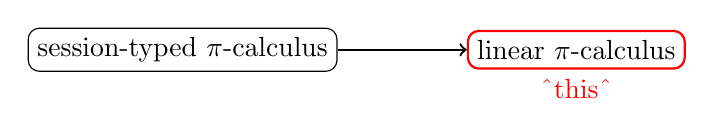
\begin{tikzpicture}
      \node[draw, rounded corners] (st) at (0,0) {session-typed \picalc{}};
      \node[draw=red, thick, rounded corners, label={[red]below:\textasciicircum this\textasciicircum}] (sh) at (5,0) {linear \picalc{}};
      \draw[->, thick] (st) -- (sh);
    \end{tikzpicture}
    \vspace{1em}

    \begin{itemize}
      \sitem untyped syntax and semantics
      \sitem must support shared channels
      \sitem goal: to prove type safety
    \end{itemize}
  \end{frame}

  \note[itemize]{
  \sitem We want to encode the session-typed \picalc{} into the linear \picalc{}
  \sitem and prove some properties of the encoding
  \sitem We first need our target language: the linear \picalc{}
  \sitem Common syntax and semantics for linear and session-typed
  }
  
  \begin{frame}{Notation}
    \begin{equation*}
      \begin{aligned}
        & \type{TYPES}          && \text{blue violet, uppercased, indices as subscripts} \\
        & \constr{constructors} && \text{burnt orange} \\
        & \func{functions}      && \text{olive green} \\
        & variables             && \text{black, in italics} \\
      \end{aligned}
    \end{equation*}
  \end{frame}

  \begin{frame}{Well-Scoped Syntax}
    \begin{mathpar}
      \inferrule
      {n : \N}
      {\constr{0} : \Var_{\suc n}}

      \inferrule
      {x : \Var_n}
      {\suc x : \Var_{\suc n}}
    \end{mathpar}

    \begin{equation*}
      \begin{aligned}
        \Process_n ::=& \; \PO_n               &&\text{(inaction)}    \\ 
        |& \; \new{} \Process_{\suc n}         &&\text{(restriction)} \\ 
        |& \; \comp{\Process_n}{\Process_n}    &&\text{(parallel)}     \\ 
        |& \; \recv{\Var_n}{}\Process_{\suc n} &&\text{(input)}       \\ 
        |& \; \send{\Var_n}{\Var_n}\Process_n  &&\text{(output)}       \\           
      \end{aligned}
    \end{equation*}

    \begin{equation*}
      \tiny
      \begin{aligned}
        & (\new{}x ) && (\comp {\recvp{x}{y} && \sendp{y}{a} && \PO} {(\new{} y) && (\sendp{x}{y} && \recvp{y}{z} && \PO)})
        && \text{names}
        \\
        & \new{} && (\comp {\recv{0} && \send{0}{a} && \PO} {\new{} && (\send{1}{0} && \recv{0} && \PO)})
        && \text{de Bruijn indices}
        \\
      \end{aligned}
    \end{equation*}
  \end{frame}

  \note[itemize]{
    \sitem \picalc{} syntax, well-scoped by construction through de Bruijn indices
    \sitem go over the constructors
  }

  \begin{frame}{Structural Congruence}
    \begin{mathpar}
      \inferrule
      { }
      {\constr{comp-assoc} : \comp{P}{(\comp{Q}{R})} \eqeq \comp{(\comp{P}{Q})}{R}}

      \inferrule
      { }
      {\constr{comp-sym} : \comp{P}{Q} \eqeq \comp{Q}{P}}
      
      \inferrule
      { }
      {\constr{comp-end} : \comp{P}{\PO_n} \eqeq P}
      
      \inferrule
      { }
      {\constr{scope-end} : \new \PO_{\suc n} \eqeq \PO_n}
      
      \inferrule
      {uQ : \Unused_{\constr{0}} \; Q}
      {\constr{scope-ext} : \new (\comp{P}{Q}) \eqeq \comp{(\new P)}{\func{lower}_{\constr{0}} \; \; Q \; uQ}}

      \inferrule
      { }
      {\constr{scope-comm} : \new \new P \eqeq \new \new \func{swap}_{\constr{0}} \; P}
    \end{mathpar}

    \centering
    $\eq{}$ is the congruent equivalence closure of $\eqeq$
  \end{frame}

  \note[itemize]{
    \sitem Parallel composition is associative, commutative and has $\PO$ as neutral element
    \sitem Garbage collection
    \sitem Scope extrusion (keep a proof $uQ$ alongside)
    \sitem Commutativity of scopes
  }

  \begin{frame}{Reduction Relation}
    \begin{mathpar}
      \inferrule
      { }
      {\constr{internal} : \Channel_n}

      \inferrule
      {i : \Var_n}
      {\constr{external} \; i : \Channel_n}

      \inferrule
      {i \; j : \Var_n \\ P : \Process_{\suc n} \\ Q : \Process_n}
      {\constr{comm} : \comp{\recv{i}P}{\send{i}{j}{Q}} \reduce{\constr{external} \; i} \comp{\func{lower}_{\constr{0}} \; (\subst{P}{\suc j}{\constr{0}}) \; uP'}{Q}}

      \inferrule
      {red : P \reduce{c} P'}
      {\constr{par} \; red : \comp{P}{Q} \reduce{c} \comp{P'}{Q}}

      \inferrule
      {red : P \reduce{c} Q}
      {\constr{res} \; red : \new P \reduce{\func{dec}\; c} \new Q}

      \inferrule
      {eq : P \eq{} P' \\ red : P' \reduce{c} Q}
      {\constr{struct} \; eq \; red : P \reduce{c} Q}
    \end{mathpar}
  \end{frame}

  \note[itemize]{
    \sitem Same scope before and after reduction
    \sitem Scope restriction is preserved (can be eliminated in strictly linear systems)
    \sitem Common channel $i$
    \sitem We keep track of $i$ at the type level
    \sitem Goes under parallel composition and scope restriction
    \sitem $\func{dec}$ saturates on $\constr{internal}$
  }

  \begin{frame}[t]
    \begin{columns}[T]
      \begin{column}{0.5\textwidth}
        \centering
        \vspace*{10em}
        untyped syntax \\
        operational semantics
        \vspace*{10em}
      \end{column}
      \vrule width 2pt
      \begin{column}{0.5\textwidth}
        \centering
        \vspace*{10em}
        \framebox{type system}
        \vspace*{10em}
      \end{column}
    \end{columns}
  \end{frame}
    
  \begin{frame}{Type System}
    \begin{itemize}
      \sitem syntax directed
      \sitem independent type and usage contexts
      \sitem extra leftover usage context
      \sitem intrinsic context splits
      \sitem based on a set of usage algebras
    \end{itemize}
  \end{frame}
  
  \note[itemize]{
  \sitem Only choice is in the types and usage annotations on scope restriction
  \sitem A syntax directed type system allows for inversion lemmas
  \sitem More on intrinsic/extrinsic later
  \sitem Linear, graded and shared types are all instances of an usage algebra
  }

  \begin{frame}{Usage Algebra}
    \begin{equation*}
    \begin{aligned}
      &\zero                  &:{} &                 &        & C \\
      &\one                   &:{} &                 &        & C \\
      &\op{\_}{\_}{\_}        &:{} &                 &        & C \to C \to C \to \Set \\
      &\func{\cdot-id^l}      &:{} &\forall x         & \to \; & \op{x}{\zero}{x} \\
      &\func{\cdot-assoc}     &:{} &\forall x y z u v & \to \; & \op{x}{y}{z} \to \op{y}{u}{v} \to \\
      &                       &    &                  &        & \type{\exists} w  \; (\op{x}{u}{w} \times \op{w}{v}{z}) \\
      &\func{\cdot-comm}      &:{} &\forall x y z     & \to \; & \op{x}{y}{z} \to \op{x}{z}{y} \\
      &\func{\cdot-min^l}     &:{} &\forall y z        & \to \; & \op{\zero}{y}{z} \to y \equiv \zero \\
      &\func{\cdot-unique}    &:{} &\forall x x' y z  & \to \; & \op{x'}{y}{z} \to \op{x}{y}{z} \to x' \equiv x \\
      &\func{\cdot-unique^l}  &:{} &\forall x y y' z  & \to \; & \op{x}{y'}{z} \to \op{x}{y}{z} \to y' \equiv y \\
      &\func{\cdot-compute^r} &:{} &\forall x y       & \to \; & \type{DEC} \; (\type{\exists} z  \; (\op{x}{y}{z})) \\
    \end{aligned}
    \end{equation*}
  \end{frame}

  \note[itemize]{
    \sitem Model as a ternary relation
    \sitem Decidable, deterministic, cancellative and has a minimal element
  }

  \begin{frame}{Capability Notation}
    \textbf{capability} input / output
    \hspace{1em}
    \textbf{multiplicity} $\zero$, $\one$, \ldots

    \begin{equation*}
      \begin{aligned}
        &C^{\func{2}} &&= C \type{\times} C \\
        &\lz          &&= \zero \comma \zero \\
        &\li          &&= \one \comma \zero \\
        &\lo          &&= \zero \comma \one \\
        &\lio         &&= \one \comma \one \\
        &\opsquared{(x_l \comma x_r)}{(y_l \comma y_r)}{(z_l \comma z_r)} &&= (\op{x_l}{y_l}{z_l}) \times (\op{x_r}{y_r}{z_r}) \\
      \end{aligned}
    \end{equation*}
  \end{frame}

  \note[itemize]{
  \sitem Notation borrowed from linear \picalc{}
  \sitem We use two carriers per channel: one for input, one for output
  }
  
  \begin{frame}{Indexed Usage Algebras}
    \begin{equation*}
      \begin{aligned}
        &\Idx               &: &\Set \\
        &\type{\exists IDX} &: &\Idx \\
        &\Usage             &: &\Idx \to \Set \\
        &\type{ALGEBRAS}    &: &(idx : \Idx) \to \Algebra_{\Usage_{idx}} \\
      \end{aligned}
    \end{equation*}

  \centering
  \begin{tabular}{l | l | l}
    & carrier & operation \\
    \hline
    \textbf{linear} & \makecell[cl]{$\constr{0} \, : \, \type{Lin}$ \\ $\constr{1} \, : \, \type{Lin}$} & \makecell[cl]{$\op{\constr{0}}{\constr{0}}{\constr{0}}$ \\ $\op{\constr{1}}{\constr{1}}{\constr{0}}$ \\ $\op{\constr{1}}{\constr{0}}{\constr{1}}$} \\
    \hline
    \textbf{graded} & \makecell[cl]{$\constr{0} \, : \type{Gra}$ \\ $\suc \, : \type{Gra} \to \type{Gra}$} & \makecell[cl]{$\forall \, x \, y \, z$ \\ $\to x \, \type{\equiv} \, y \, \func{+} \, z$ \\ $\to \op{x}{y}{z}$} \\
    \hline
    \textbf{shared} & $\constr{\omega} \, : \, \type{Sha}$ & $\op{\constr{\omega}}{\constr{\omega}}{\constr{\omega}}$ \\
  \end{tabular}
  \end{frame}

  \note[itemize]{
    \sitem Lump multiple algebras together
  }
  
  \begin{frame}{Types}
    \begin{mathpar}
      \inferrule
      { }
      {\unit : \Type}

      \inferrule
      {n : \N}
      {\base{n} : \Type}
      
      \inferrule
      {t : \Type \\ \stacked{idx : \Idx \\\\ x : \Usage_{idx}^{\func{2}}}}
      {\channel{t}{x} : \Type}
    \end{mathpar}

    \centering
    \vfill{}
    \textit{e.g.} $\channel{\channel{\unit}{\omega}}{\li}$
  \end{frame}

  \begin{frame}{Typing Relation}
    \begin{description}
    \item [$\PreCtx_n$] list of $\Type$s of length $n$
    \item [$\Idxs_n$] list of $\Idx$s of length $n$
    \item [$\Ctx_{idxs}$] list of $\Usage^{\func{2}}$s indexed over $idxs  \; : \Idxs_n$
    \end{description}
    
    \small
    \begin{mathpar}
    \datatype{
      \gamma : \PreCtx_n \\
      \stacked{
        idxs : \Idxs_n \\\\
        \Gamma : \Ctx_{idxs}} \\
      P : \Process_n \\
      \Delta : \Ctx_{idxs}}
    {\types{\gamma}{\Gamma}{P}{\Delta} : \Set}
    \end{mathpar}
  \end{frame}

  \note[itemize]{
  \sitem Typing judgment through typing relations
  \sitem One relation on processes, one relation on variable references (omitted for brevety)
  \sitem Relation on variable references uses the monoid to split multiplicities
  }
  
  \begin{frame}{Typing Rules}
    \begin{mathpar}
      \inferrule
    {l \hspace{0.1em} : \types{\gamma}{\Gamma \hspace{0.3em}}{P}{\Delta} \\\\
      r : \types{\gamma}{\Delta}{Q}{\Xi}}
    {\constr{comp} \; l \; r : \types{\gamma}{\Gamma}{\comp{P}{Q}}{\Xi}}

    \inferrule
    { }
    {\constr{end} : \types{\gamma}{\Gamma}{\PO}{\Gamma}}
  
    \end{mathpar}
  \end{frame}
  
  \note[itemize]{
  \sitem Instead of one authoritative context split, give decision power to P
  }

  \begin{frame}{Typing Rules}
    \begin{mathpar}
    \inferrule
    {t : \Type \\ x : \Usage_{idx}^{\func{2}} \\ y : \Usage_{idx'} \\\\
      cont : \types{\gamma \comma \channel{t}{x}}{\Gamma \comma (y \comma y) }{P}{\Delta \comma \lz}}
    {\constr{chan} \; t \; x \; y \; cont : \types{\gamma}{\Gamma}{\new P}{\Delta}}

    \inferrule
        {\stacked{
            chan_i : \contains{\gamma \hspace{1.1em}}{\Gamma \hspace{1.5em}}{i}{\channel{t}{x}}{\li}{\Xi} \\\\
            cont \hspace{0.4em} : \types{\gamma \comma t}{\Xi \comma x}{P \hspace{4.6em}}{\Theta \comma \lz}}}
        {\constr{recv} \; chan_i \; cont : \types{\gamma}{\Gamma}{\recv{i}{P}}{\Theta}}
  
    \inferrule
        {\ldots}
        {\constr{send} \; \ldots}
  
    \end{mathpar}
  \end{frame}

  \note[itemize]{
  \sitem Newly introduced channels are balanced
  \sitem The multiplicities of new variables must be exhausted
  }

  \begin{frame}{Failed Efforts}
    \begin{itemize}
    \sitem using functions to update usage contexts
      \begin{mathpar}
        \inferrule
        {\ldots \\ (\func{update}_i \; \ldots \; \Gamma) \vdash P \\ \ldots}
        {\Gamma \; \type{\vdash} \; \recv{i}{P}}
      \end{mathpar}
    \sitem extrinsic context splits
      \begin{mathpar}
        \inferrule
        {\opctx{\Gamma}{\Delta}{\Xi} \\\\
         \Delta \; \type{\vdash} P \\\\
         \Xi \; \type{\vdash} Q}
        {\Gamma \; \type{\vdash} \; \comp{P}{Q}}
      \end{mathpar}
    \end{itemize}
  \end{frame}

  \note[itemize]{
  \sitem The extrinsic context split is authoritative, P already knows what it needs
  }

  \begin{frame}[t]
    \begin{columns}[T]
      \begin{column}{0.5\textwidth}
        \centering
        \vspace*{10.5em}
        type system
        \vspace*{10em}
      \end{column}
      \vrule width 2pt
      \begin{column}{0.5\textwidth}
        \centering
        \vspace*{10em}
        \framebox{type safety}
        \vspace*{10em}
      \end{column}
    \end{columns}
  \end{frame}
  
  \begin{frame}{Subject Congruence}
    \begin{itemize}
      \setlength\itemsep{1em}
      \sitem \textbf{framing} the only resources the well-typedness of a process depends on are the ones used by it.

      \sitem \textbf{weakening} inserting a new variable into the context preserves the well-typedness of a process as long as the usage annotation of the inserted variable is preserved as a leftover.

      \sitem \textbf{strengthening} removing an unused variable preserves the well-typedness of a process.

      \sitem \textbf{subject congruence} applying structural congruence rules to a well typed process preserves its well-typedness.
    \end{itemize}
  \end{frame}

  \note[itemize]{
  \sitem First three by induction on \textsc{Types} and \textsc{VarRef}
  \sitem First three state for the first time for the \picalc{}
  }

  \begin{frame}{Subject Reduction}
    \begin{itemize}
      \setlength\itemsep{2em}
      \sitem \textbf{substitution} \\
      substituting a variable $i$ for a variable $j$ in a well-typed process $P$ results in a well-typed process as long as the leftovers at index $j$ after $P$ are at least the consumption made by $P$ at index $i$.

      \sitem \textbf{subject reduction} \\
      let $\types{\gamma}{\Gamma}{P}{\Xi}$ and $P \reduce{c} Q$,
      \begin{itemize}
        \sitem if $c$ is $\constr{internal}$, then $\types{\gamma}{\Gamma}{Q}{\Xi}$.
        \sitem if $c$ is $\constr{external} \; i$ and $\containsusage{\Gamma}{i}{\lio}{\Delta}$, then $\types{\gamma}{\Delta}{Q}{\Xi}$.
      \end{itemize}
    \end{itemize}
  \end{frame}

  \begin{frame}{Future Work}
    \begin{itemize}
    \sitem prove preservation of well-balancedness
    \sitem product types
    \sitem sum types
    \sitem recursion
    \sitem bidirectional type system
    \sitem decidable type checking
    \sitem use as target language for the session-typed \picalc{}
    \end{itemize}
  \end{frame}

  \begin{frame}
    \centering
    \Huge{thank you!} \\
    \Huge{\textasciicircum{}\_\textasciicircum{}} \\
    \Huge{questions?}
  \end{frame}
    

  %%%%%%%%%%%%%%%%%%%%%%%%%%%%%%%%%%%%%%%%%%%%%%%%%%%%%%%%%%%%%%%%%%%%%%%%%%%%%%%%%%
  

  \begin{frame}{Variable References}
    \begin{mathpar}
      {\tiny
      \datatype{
        \gamma : \PreCtx_n \\
        \stacked{
          idxs : \Idxs_n \\\\
          \Gamma : \Ctx_{idxs}} \\
        i : \Var_n \\
        t : \Type \\
        \stacked{
          idx : \Idx \\\\
          y : \Usage_{idx}^{\func{2}}} \\
        \Delta : \Ctx_{idxs}}
      {\contains{\gamma}{\Gamma}{i}{t}{y}{\Delta} : \Set}}

      \inferrule
      {\opsquared{x}{y}{z}}
      {\constr{0} : \contains{\gamma \comma t}{\Gamma \comma x}{\constr{0}}{t}{y}{\Gamma \comma z}}
      
      \inferrule
      {\hspace{-0.1em} loc_i : \contains{\gamma \hspace{1.4em}}{\Gamma \hspace{1.7em}}{\hspace{1em} i}{t}{x}{\Delta}}
      {\suc \; loc_i : \contains{\gamma \comma t'}{\Gamma \comma x'}{\suc i}{t}{x}{\Delta \comma x'}}
    \end{mathpar}
  \end{frame}

  \note[itemize]{
  \sitem Constructor completely determined by $i$
  \sitem User alleviated from proof burden $\opsquared{x}{y}{z}$, which can be computed given $x$ and $y$
  }
  
  \begin{frame}{Type Safety: Substitution}
    \textbf{Substitution with accumulator} \\
      Let $\types{\gamma}{\Gamma_i}{P}{\Psi_i}$.
      Let there be some $\Gamma$, $\Psi$, $\Gamma_j$ and $\Psi_j$ such that:
      \setlength{\linewidth}{.8\linewidth}
      \begin{multicols}{2}
        \begin{itemize}
        \sitem $\contains{\gamma}{\Gamma_i}{i}{t}{m}{\Gamma}$
        \sitem $\contains{\gamma}{\Gamma_j}{j}{t}{m}{\Gamma}$
        \sitem $\contains{\gamma}{\Psi_i}{i}{t}{n}{\Psi}$
        \sitem $\contains{\gamma}{\Psi_j}{j}{t}{n}{\Psi}$
        \end{itemize}
        \vfill\null
        \columnbreak
        \scriptsize
        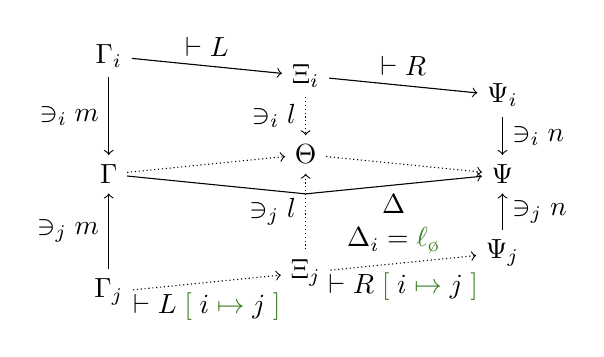
\begin{tikzpicture}
          \node (gamma-i) at (0,3)   {$\Gamma_i$};
          \node (gamma-m) at (0,1.5)   {$\Gamma$};
          \node (gamma-j) at (0,0)   {$\Gamma_j$};
          \node (xi-i)    at (2.5,2.75) {$\Xi_i$};
          \node (theta)   at (2.5,1.75) {$\Theta$};
          \node (delta-m) at (2.5,1.25) {};
          \node (xi-j)    at (2.5,0.25) {$\Xi_j$};
          \node (psi-i)   at (5,2.5)   {$\Psi_i$};
          \node (psi-m)   at (5,1.5)   {$\Psi$};
          \node (psi-j)   at (5,0.5)   {$\Psi_j$};

          \draw[-]  (gamma-m) -- (delta-m.center);
          \draw[->] (delta-m.center) -- node[align=center,below] {$\Delta$\\$\Delta_i = \lz$}(psi-m);

          \draw[->,densely dotted] (gamma-m) -- (theta);
          \draw[->,densely dotted] (theta) -- (psi-m);
          
          \draw[->] (gamma-i) -- node[left] {$\ni_i m$} (gamma-m);
          \draw[->] (gamma-j) -- node[left] {$\ni_j m$} (gamma-m);
          \draw[->] (psi-i) -- node[right] {$\ni_i n$} (psi-m);
          \draw[->] (psi-j) -- node[right] {$\ni_j n$} (psi-m);

          \draw[->] (gamma-i) -- node[above] {$\vdash L$} (xi-i);
          \draw[->] (xi-i) -- node[above] {$\vdash R$} (psi-i);
          \draw[->,densely dotted] (gamma-j) -- node[below] {$\vdash \subst{L}{j}{i}$} (xi-j);
          \draw[->,densely dotted] (xi-j) -- node[below] {$\vdash \subst{R}{j}{i}$} (psi-j);
          \draw[->,densely dotted] (xi-i) -- node[left] {$\ni_i l$} (theta);
          \draw[->,densely dotted] (xi-j) -- node[left] {$\ni_j l$} (theta);
        \end{tikzpicture}
      \end{multicols}
      Let there be some $\Delta$ such that $\opctx{\Gamma}{\Delta}{\Psi}$.
      Let $\Delta$ have usage $\lz$ at position $i$.
      Then $\types{\gamma}{\Gamma_j}{\subst{P}{j}{i}}{\Psi_j}$.
  \end{frame}
\end{document}